% Section: Kernel
\section{Kernel choice} \label{sec:autokernel}
Choosing an appropriate \emph{Kernel Function} in a regression problem has always been a nightmare for researchers and analysts. In this section, from the practical meaning of a \emph{Kernel Function}, we introduce an automatic way to construct a desired composite form of \emph{Kernel}.
We also introduce a special \emph{Additive Kernel} used specifically for an Additive Gaussian Process, which is a case we will be solving in our experiment (Section~\ref{sec:experiment}).
This section is based on the work of Duvenaud and Lloyd et. al \cite{duvenaud2013structure,lloyd2014automatic,duvenaud2014automatic,duvenaud2011additive}.


\subsection{Kernels express structures}

%% Base Kernels

\para{Base Kernels}
As we all know, different kernels can represent different kinds of data. In Figure~\ref{fig:singlekernel}, we show 4 different kinds of base kernels, each represents a specific kind of data characteristics (Table~\ref{tab:kernel}). Each function of the kernel is shown in Equation~\ref{eqa:kernel}


\begin{equation}
\left \{
\begin{aligned} \label{eqa:kernel}
k_{LIN}(x,x^{'}) &= \sigma_{b}^{2} + \sigma_{v}^{2} (x-l)(x^{'}-l) 	\\
k_{SE}(x,x^{'}) &= \sigma^2 exp(-\frac{(x-x^{'})^2}{2l^2})	\\
k_{PER}(x,x^{'}) &= \sigma^2 exp(-\frac{2sin^2 (\pi(x-x^{'})/p)}{l^2})	\\
k_{RQ}(x,x^{'}) &= \sigma^2 (1+\frac{(x-x^{'})^2}{2\alpha l^2})^{-\alpha}	\\
\end{aligned}
\right.
\end{equation}


\begin{figure}[htp]
\begin{minipage}[htp]{1\linewidth}
	\centering
  	\subfloat[Linear(LIN)]{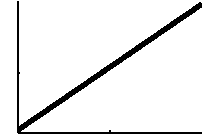
\includegraphics[width=0.45\textwidth]{figure/kernels/lin_kernel.pdf}}
	\subfloat[Squared exp(SE)]{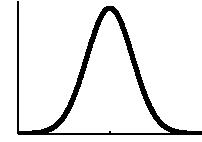
\includegraphics[width=0.45\textwidth]{figure/kernels/se_kernel.pdf}}\\
	\subfloat[Periodic(PER)]{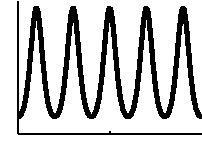
\includegraphics[width=0.45\textwidth]{figure/kernels/per_kernel.pdf}}
	\subfloat[Rational quadratic(RQ)]{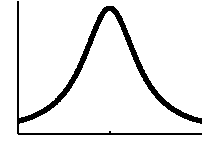
\includegraphics[width=0.45\textwidth]{figure/kernels/rq_kernel.pdf}}
% \vspace{-0.1in}
\caption{Base Kernels}
\label{fig:singlekernel} % FIG1
\end{minipage}
\vspace{-0.05in}
\end{figure}


\begin{table}[htp]
\centering
{\small
\begin{tabular}{c|c}
    \hline
    \textbf{Kernel} & \textbf{Data Structures} \\ 
    \hline
	   Linear(LIN) & linear functions\\
	   Squared exponential(SE) & local variation\\
	   Periodic(PER) & repeating structure\\
	   Rational quadratic(RQ) & multi-scale variation\\
	   \hline
\end{tabular}
}
\caption{Different kinds of kernels and its represented data structures.}
\label{tab:kernel}
% \vspace{-0.05in}
\end{table}



%% Compositional Kernels
\para{Compositional Kernels}
When the data structure we are dealing with is not contained in any of the above base kernel, we have to made one to fit the targeted data characteristics. A possible and probable approach of making a customized kernel is to do some addition and multiplication to the base kernels.
\begin{align}
k_{k_{a} + k_{b}} (\textbf{x}, \textbf{x}^{'}) &= k_{a} (\textbf{x}, \textbf{x}^{'}) + k_{b} (\textbf{x}, \textbf{x}^{'}) \\
k_{k_{a} \times k_{b}} (\textbf{x}, \textbf{x}^{'}) &= k_{a} (\textbf{x}, \textbf{x}^{'}) \times k_{b} (\textbf{x}, \textbf{x}^{'})
\end{align}
By addition and multiplication, we are able to construct some very complicated data structure.
Below, we show some examples of structures by compositional kernels (Figure~\ref{fig:compKernel}) and the data structures they are capable of representing (Table~\ref{tab:compKernel}).


\begin{figure}[htp]
\begin{minipage}[htp]{1\linewidth}
	\centering
  	\subfloat[LIN + PER]{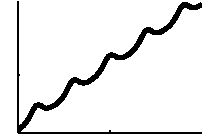
\includegraphics[width=0.45\textwidth]{figure/kernels/lin_plus_per.pdf}}
	\subfloat[SE + PER]{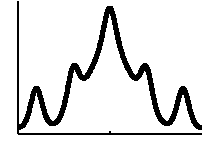
\includegraphics[width=0.45\textwidth]{figure/kernels/se_plus_per.pdf}}\\
	\subfloat[SE $\times$ PER]{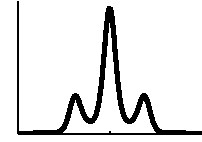
\includegraphics[width=0.45\textwidth]{figure/kernels/se_times_per.pdf}}
	\subfloat[LIN $\times$ LIN]{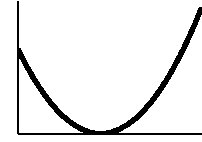
\includegraphics[width=0.45\textwidth]{figure/kernels/lin_times_lin.pdf}}
% \vspace{-0.1in}
\caption{Some examples of the compositional kernels}
\label{fig:compKernel} % FIG1
\end{minipage}
\vspace{-0.05in}
\end{figure}


\begin{table}[htp]
\centering
{\small
\begin{tabular}{c|c}
    \hline
    \textbf{Kernel} & \textbf{Data Structures} \\ 
    \hline
	   LIN+ PER & periodic plus trend\\
	   SE + PER & periodic plus noise\\
	   SE $\times$ PER & locally periodic\\
	   LIN $\times$ LIN & quadratic functions\\
	   \hline
\end{tabular}
}
\caption{Some examples of the compositional kernels}
\label{tab:compKernel}
% \vspace{-0.05in}
\end{table}


\subsection{Automatic Construction} \label{sec:autokernel}
As we can see in the above analysis, choice of the form of a \emph{Kernel Function} can be critical in a GPR. However, this process was used to be a privileged work for experts since it requires a whole lot of experience and expertise. In \cite{duvenaud2013structure,lloyd2014automatic,duvenaud2014automatic}, Duvenaud and Lloyd et.al describe a tractable method to let a computer be capable of doing this work.
This procedure is summarized as follows:

\para{Kernel Family}
We consider the \emph{base kernels} as shown in Figure~\ref{fig:singlekernel}, any algebraic expression using these kernels as a combination of $+$ and $\times$ could be our target. And any of our target with the concatenation of the parameters forms a kernel family.

\para{Scoring a Kernel Family}
We must find a way to evaluate a kernel family. At here, we use the marginal likelihood\cite{blumer1987occam} as our criterion, and use the Bayesian Information Criterion(BIC)\cite{schwarz1978estimating} to approximate the integration over kernel parameters.

\para{Search over structures}
Last, by using a greedy search: At each stage, expand the current kernel by all possible \emph{operators}
and choose the highest scoring one. The number of working stage is defined by user.
Possible operators are listed as follows:
\begin{enumerate}
	\item Any expression $S$ can be replaced by $S + B$
	\item Any expression $S$ can be replaced by $S \times B$
	\item Any base kernel $B$ can be replaced by $B^{'}$
\end{enumerate}
where $B$ and $B^{'}$ represent any base kernel family. Note that, in the work \cite{lloyd2014automatic}, Lloyd et. al also take account of the changepoint operator $CP$, the changewindow operator $CW$, and some empirical operators. They also add some base kernels to improve the algorithm. Due to limited time and space, we only introduce the most important part here.

The implemented Matlab and Python code by Duvenaud and Lloyd et.al can be found on github\footnote{Available at \color{blue}\href{http://github.com/jamesrobertlloyd/gpss-research}{github.com/jamesrobertlloyd/gpss-research} \color{black} and \color{blue}\href{http://github.com/jamesrobertlloyd/gp-structure-search}{github.com/jamesrobertlloyd/gp-structure-search}.}.

\begin{algorithm}[t]
        \caption{Automatic kernel construction algorithm}
        \begin{algorithmic}
        		\Require Required search depth $N$
        		\State Initialize kernel $S$
            	\For{$t = 1 \to N$}
			\State $CurScore \gets 0$
			\For{$ Possible ~ operators ~ S^{'}$}
	            		\If {Score(S) > CurScore}
					\State $S \gets S^{'}$
				\EndIf
			\EndFor
	    	\EndFor
		\State \Return $kernel~S$
       	\end{algorithmic}
\end{algorithm}


\subsection{Additive Gaussian Processes}

\para{Additive Gaussian Process}
\cite{duvenaud2011additive}
In some 


\para{Additive Kernels}
We now give the precise definition of additive kernels.
As shown in \cite{duvenaud2011additive}, we define the 1st, 2nd, nth order additive kernel as:
\begin{align}
k_{add_{1}} (\textbf{x},\textbf{x}^{'}) &= \sigma^2_1 \sum_{i=1}^{D} k_{i} (\textbf{x}_{i},\textbf{x}_{i}^{'}) \\
k_{add_{2}} (\textbf{x},\textbf{x}^{'}) &= \sigma^2_2 \sum_{i=1}^{D} \sum_{j=i+1}^{D} k_{i} (\textbf{x}_{i},\textbf{x}_{i}^{'}) k_{j} (\textbf{x}_{j},\textbf{x}_{j}^{'}) \\
k_{add_{n}} (\textbf{x},\textbf{x}^{'}) &= \sigma^2_n \sum_{1 \leqslant i_1 < i_2 < ... < i_n \leqslant D} ( \prod_{d=1}^{n} k_{i_d} (\textbf{x}_{i_d},\textbf{x}_{i_d}^{'}) ) \\
\end{align}
where $k_{i} (\textbf{x}_{i},\textbf{x}_{i}^{'})$ is the \emph{base kernel} we assigned at first for each dimension $i \in \{1,2,...,D\}$.
A full additive kernel is a sum of all orders' additive kernels, as in equation~\ref{eqa:add}:
\begin{equation} \label{eqa:add}
K_{add_{full}} (\textbf{x},\textbf{x}^{'}) = \sum_{n=1}^{D} k_{add_{n}} (\textbf{x},\textbf{x}^{'})
\end{equation}
In the real practice, we could choose specific orders of the additive kernels:
\begin{equation} \label{eqa:add}
K_{add_{prac}} (\textbf{x},\textbf{x}^{'}) = \sum_{n} k_{add_{n}} (\textbf{x},\textbf{x}^{'})
\end{equation}

We also noted that if every base kernel is a one-dimensional squared-exponential(SE) kernal, the Dth order term of the additive kernel would be:
\begin{equation} \label{eqa:add}
\begin{aligned}
K_{add_{D}} (\textbf{x},\textbf{x}^{'}) &= \sigma_{D}^{2} \prod_{d=1}^D k_{d} (\textbf{x}_{d},\textbf{x}_{d}^{'}) \\
		     &= \sigma_{D}^{2} \prod_{d=1}^D exp(-\frac{(\textbf{x}_{d}-\textbf{x}_{d}^{'})^{2}}{2l_{d}^{2}}) \\
		     &= \sigma_{D}^{2}  exp(-\sum_{d=1}^{D} \frac{(\textbf{x}_{d}-\textbf{x}_{d}^{'})^{2}}{2l_{d}^{2}})
\end{aligned}
\end{equation}
which is just the multivariate squared-exponential kernel.















